\chapter{Метрики, расширение и первая космология}

К концу предыдущей лекции мы пришли к лоренц-инвариантному волновому уравнению и готовились записать уравнения Максвелла в пространственно-временной форме. Вопрос из аудитории дает теперь полезное предостережение, прежде чем мы перейдем к гравитации: какую часть физической теории симметрия может определить сама по себе? Ответ однозначен: очень многое, но не всё. Лоренц-инвариантность — мощный фильтр для возможных законов. Она не заменяет ни остальных физических предположений, ни эксперимента.

\section{Что симметрия не определяет}

\begin{classroomqa}
\audiencequestion{Если уже известно, что электрическое и магнитное поля совместно преобразуются при преобразованиях Лоренца, следуют ли уравнения Максвелла из одной только теории относительности?}
\lecturerresponse{Нет. Теория относительности накладывает ограничения на форму уравнений, но при их построении используются также линейность уравнений, низкий порядок содержащихся в них производных, способ преобразования полей и экспериментальная информация. Без этих дополнительных составляющих по-прежнему были бы возможны многие лоренц-ковариантные полевые уравнения.}
\end{classroomqa}

Наиболее важное из этих дополнительных предположений для начального обсуждения — линейность. Если \(A(x,t)\) является решением линейного полевого уравнения, то \(\lambda A(x,t)\) тоже является решением при любой постоянной \(\lambda\). Если \(A\) и \(B\) — решения, то решением будет и
\begin{equation}
  C(x,t)=A(x,t)+B(x,t).
  \label{eq:superposition}
\end{equation}
Это принцип суперпозиции. Две электромагнитные волны без источников могут проходить друг через друга и оставаться неизменными. Они не сталкиваются непосредственно так, как материальные объекты. Они могут косвенно взаимодействовать через заряженное вещество, потому что каждая волна приводит заряды в движение, а движущиеся заряды излучают, но сами вакуумные полевые уравнения линейны.

\begin{figure}[H]
\centering
\includegraphics[width=0.64\textwidth]{lecture_08_figure_01.png}
\caption{Два волновых профиля на доске при обсуждении суперпозиции. Их сумма снова является допустимой волной без источников.}
\lectureframe{00:05:30}
\end{figure}

Гармонический осциллятор делает алгебру наглядной. Предположим, что
\begin{equation}
  m\ddot x=-kx.
  \label{eq:linear-oscillator}
\end{equation}
Если \(x_1\) и \(x_2\) удовлетворяют \eqref{eq:linear-oscillator}, то
\begin{equation}
  m(\ddot x_1+\ddot x_2)
  =-k(x_1+x_2),
\end{equation}
следовательно, \(x_1+x_2\) является решением. Однако добавим нелинейный член,
\begin{equation}
  m\ddot x=-kx+p x^2,
  \label{eq:nonlinear-oscillator}
\end{equation}
и сумма перестает работать:
\begin{equation}
  (x_1+x_2)^2=x_1^2+x_2^2+2x_1x_2.
\end{equation}
Перекрестный член \(2x_1x_2\) не имеет аналога в двух отдельных уравнениях. Теперь два движения влияют друг на друга.

\begin{figure}[H]
\centering
\includegraphics[width=0.73\textwidth]{lecture_08_figure_02.png}
\caption{Отдельные уравнения осциллятора в сравнении с уравнением для их суммы. Квадратичный член выявляет дополнительный перекрестный член, нарушающий суперпозицию.}
\lectureframe{00:10:10}
\end{figure}

Этот пример закрепляет методологический тезис, который будет оставаться в силе на протяжении всего обсуждения космологии. Симметрия говорит нам, какие величины можно комбинировать и какие уравнения допустимы. Динамика и наблюдение говорят нам, какое из допустимых уравнений использует природа.

\section{Интервал как геометрия}

Теперь мы оставим электромагнетизм и кратким путем перейдем к общей теории относительности и космологии. Исходным объектом служит интервал между соседними событиями. Обозначим событие четырьмя координатами \(x^\mu\), а близкое к нему событие — \(x^\mu+dx^\mu\). В инерциальных декартовых координатах, при \(c=1\) и соглашении о сигнатуре \((+,-,-,-)\),
\begin{equation}
  d\tau^2
  =dt^2-dx^2-dy^2-dz^2
  =dx^\mu dx_\mu
  =\eta_{\mu\nu}\,dx^\mu dx^\nu.
  \label{eq:minkowski-interval}
\end{equation}
Инвариантной величиной является \(d\tau^2\), а не какая-либо одна разность координат. Преобразования Лоренца изменяют \(dt,dx,dy,dz\), сохраняя эту квадратичную комбинацию. Поэтому специальную теорию относительности можно рассматривать как геометрию пространства-времени Минковского.

\begin{figure}[H]
\centering
\includegraphics[width=0.72\textwidth]{lecture_08_figure_03.png}
\caption{Интервал Минковского, последовательно записанный в компонентной записи, в записи со свернутыми индексами и в записи через метрический тензор.}
\lectureframe{00:14:50}
\end{figure}

Простота \eqref{eq:minkowski-interval} зависит от координат. Даже плоская плоскость может получить непривычные коэффициенты, если мы введем на ней неудачные координаты. Пусть \(x\) измеряется в сантиметрах, а \(y\) — в метрах. Тогда для физического смещения
\begin{equation}
  ds^2=dx^2+\left(\frac{dy}{100}\right)^2
      =dx^2+10^{-4}dy^2.
  \label{eq:mixed-units}
\end{equation}
Множитель \(10^{-4}\) ничего не говорит о кривизне. Он лишь переводит одни единицы в другие.

\begin{figure}[H]
\centering
\includegraphics[width=0.59\textwidth]{lecture_08_figure_04.png}
\caption{Плоская плоскость, описанная так, что на одной оси используются сантиметры, а на другой — метры. Неравные коэффициенты метрики кодируют единицы измерения, а не кривизну.}
\lectureframe{00:20:10}
\end{figure}

Косоугольные координаты добавляют смешанный член. В двух измерениях наиболее общую локальную квадратичную форму можно записать как
\begin{align}
  ds^2
  &=a_{11}\,dx^2+a_{12}\,dx\,dy\notag\\
  &\quad+a_{21}\,dy\,dx+a_{22}\,dy^2,
  \qquad a_{12}=a_{21}.
  \label{eq:quadratic-form}
\end{align}
Поскольку обычные дифференциалы коммутируют, \(dx\,dy=dy\,dx\), вклад вносит только симметричная часть массива коэффициентов. Соберем коэффициенты в матрицу
\begin{equation}
  g=
  \begin{pmatrix}
    a_{11} & a_{12}\\
    a_{21} & a_{22}
  \end{pmatrix}.
  \label{eq:metric-matrix}
\end{equation}
Эта матрица — \emph{метрика}. Она задает локальное правило, переводящее разности координат в физические интервалы.

\begin{figure}[H]
\centering
\includegraphics[width=0.71\textwidth]{lecture_08_figure_05.png}
\caption{Квадратичная дифференциальная форма и ее симметричная матрица коэффициентов \(2\times2\) в тот момент, когда эта матрица отождествляется с метрикой.}
\lectureframe{00:24:07}
\end{figure}

Однородные прямоугольные или косоугольные координатные сетки дают постоянные коэффициенты. Если координатные линии искривляются, сгущаются или расходятся, эти коэффициенты становятся функциями положения, даже когда сама поверхность остается плоской. Общая запись для пространства-времени имеет вид
\begin{equation}
  ds^2=g_{\mu\nu}(x)\,dx^\mu dx^\nu.
  \label{eq:general-metric}
\end{equation}

\begin{figure}[H]
\centering
\includegraphics[width=0.66\textwidth]{lecture_08_figure_06.png}
\caption{Общая метрика, зависящая от положения, после того как координатной сетке позволено меняться от точки к точке.}
\lectureframe{00:28:10}
\end{figure}

Зная \(g_{\mu\nu}\) в заданной системе координат, мы определяем локальные расстояния, времена и углы, а тем самым и геометрию. Обратное соответствие неоднозначно: одна и та же геометрия имеет бесконечно много координатных описаний, а значит, бесконечно много наборов коэффициентных функций, связанных преобразованиями координат.

\section{Координатная сложность и внутренняя кривизна}

Теперь мы должны отличать сложную метрику от искривленного пространства. Сверните лист бумаги в цилиндр, не растягивая его. Его вид в комнате изменится, но все расстояния, измеряемые на листе, останутся теми же. Существо, ограниченное этой бумагой, не сможет обнаружить изгиб никаким внутренним измерением. Это внешнее изгибание, а не та кривизна, которую мы имеем здесь в виду.

Полусфера иная. Ее нельзя расплющить в плоскость без растяжения, разрыва или сжатия. Плоская карта Земли неизбежно искажает либо расстояния, либо площади, либо углы, либо какую-то их комбинацию. Это препятствие является внутренним и может быть обнаружено без обращения к окружающему пространству.

Полярные координаты дают необходимый плоский контрпример. На плоскости бесконечно малое радиальное смещение имеет длину \(dr\), тогда как угловое смещение \(d\theta\) при радиусе \(r\) имеет длину \(r\,d\theta\). Поэтому
\begin{equation}
  ds^2=dr^2+r^2d\theta^2,
  \qquad
  g_{\text{polar}}=
  \begin{pmatrix}
    1&0\\
    0&r^2
  \end{pmatrix}.
  \label{eq:polar-metric}
\end{equation}
Коэффициент \(r^2\) меняется по плоскости, и все же плоскость остается плоской. Замена переменных
\begin{equation}
  x=r\cos\theta,\qquad y=r\sin\theta
\end{equation}
возвращает постоянную метрику \(ds^2=dx^2+dy^2\).

\begin{figure}[H]
\centering
\includegraphics[width=0.70\textwidth]{lecture_08_figure_07.png}
\caption{Полярная метрика и ее возвращение к декартовой метрике. Зависящая от положения матрица слева по-прежнему описывает плоскость.}
\lectureframe{00:39:20}
\end{figure}

\begin{classroomqa}
\audiencequestion{Должно ли угловое расстояние в полярных координатах содержать синус?}
\lecturerresponse{Не на плоскости. Там длина дуги равна \(r\,d\theta\). Синус появляется на сфере, где окружность широты имеет радиус \(R\sin\theta\).}
\end{classroomqa}

Рассмотрим сферу радиуса \(R\). Пусть \(\theta\) — полярный угол, отсчитываемый от северного полюса, а \(\phi\) — азимутальный угол. Шаг вдоль меридиана имеет длину \(R\,d\theta\). При полярном угле \(\theta\) окружность широты имеет радиус \(R\sin\theta\), поэтому азимутальный шаг имеет длину
\(R\sin\theta\,d\phi\). Локальная теорема Пифагора дает
\begin{align}
  ds^2
  &=R^2\left(d\theta^2+\sin^2\theta\,d\phi^2\right),
  \label{eq:sphere-metric}\\
  g_{\text{sphere}}=
  &\begin{pmatrix}
    R^2&0\\
    0&R^2\sin^2\theta
  \end{pmatrix}.
\end{align}

\begin{figure}[H]
\centering
\includegraphics[width=0.72\textwidth]{lecture_08_figure_08.png}
\caption{Сфера, ее угловой линейный элемент и соответствующая матрица метрики. Множитель \(\sin^2\theta\) отражает сужающиеся окружности широты.}
\lectureframe{00:45:15}
\end{figure}

\begin{figure}[H]
\centering
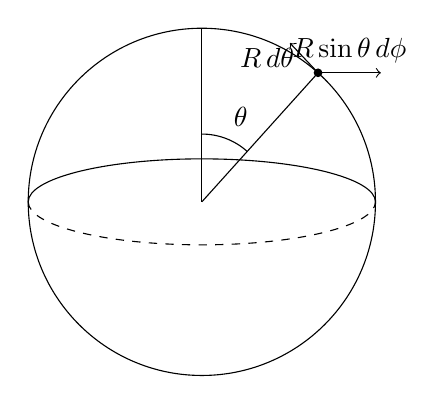
\begin{tikzpicture}[scale=1.05]
  \draw (0,0) circle (2.1);
  \draw[dashed] (-2.1,0) arc (180:360:2.1 and 0.52);
  \draw (2.1,0) arc (0:180:2.1 and 0.52);
  \coordinate (P) at (48:2.1);
  \fill (P) circle (1.5pt);
  \draw (0,0) -- (0,2.1);
  \draw (0,0) -- (P);
  \draw (0,0.82) arc (90:48:0.82);
  \node at (0.47,1.03) {\(\theta\)};
  \draw[->] (P) -- ++(-0.34,0.36)
    node[midway,left] {\(R\,d\theta\)};
  \draw[->] (P) -- ++(0.76,0)
    node[midway,above] {\(R\sin\theta\,d\phi\)};
\end{tikzpicture}
\caption{Аккуратное восстановление локальных дифференциальных катетов, использованных для получения \eqref{eq:sphere-metric}.}
\end{figure}

Никакая глобальная замена координат не превращает \eqref{eq:sphere-metric} в постоянную евклидову матрицу. Двумерный наблюдатель может обнаружить это внутренним образом: у достаточно большого треугольника, образованного геодезическими, сумма углов больше \(180^\circ\). Тем самым мы пришли к полезному критерию. Переменные коэффициенты сами по себе не влекут кривизны. Кривизна — это препятствие к нахождению координат, делающих метрику постоянной во всей рассматриваемой области.

\section{От искривленного пространства-времени к космологии}

Общая теория относительности допускает, что само пространство-время может обладать этой внутренней кривизной. Зависимость \(g_{\mu\nu}\) от положения все еще может быть артефактом координат, как в полярных координатах, но в действительно искривленном пространстве-времени никакое преобразование координат не устраняет эту зависимость глобально.

\begin{figure}[H]
\centering
\includegraphics[width=0.70\textwidth]{lecture_08_figure_09.png}
\caption{Переход от частных координатных примеров к общему линейному элементу пространства-времени \(ds^2=g_{\mu\nu}(x)dx^\mu dx^\nu\).}
\lectureframe{00:48:40}
\end{figure}

Мы не будем обращаться ко всему аппарату уравнений Эйнштейна. Вместо этого ограничимся геометриями, подходящими для космологии: пространство считается однородным на достаточно больших масштабах, тогда как геометрия может меняться со временем. Однородность означает, что ни одно место не выделено по сравнению с другим. Это не означает плоскостности: каждая точка на сфере эквивалентна любой другой, и всё же сфера искривлена. И это также не означает отсутствия структуры на всех масштабах.

\begin{classroomqa}
\audiencequestion{Как Вселенная может быть однородной, если галактики образуют скопления, стены и филаменты?}
\lecturerresponse{Речь идёт о масштабах после грубого усреднения. Звёзды, галактики и скопления сильно неоднородны. Если сравнивать области размером в сотни миллионов световых лет, эти структуры в среднем приближаются к однородному распределению. Космологический принцип — это эмпирическая рабочая гипотеза, а не логическая необходимость; достаточно большие систематические различия, включая различия по направлениям в космическом фоне, могли бы её опровергнуть.}
\end{classroomqa}

Вторая крупномасштабная предпосылка этой лекции — пространственная плоскостность. В фиксированный космический момент достаточно большие треугольники выглядят евклидовыми: сумма их углов равна \(180^\circ\). Это утверждение о геометрии трёхмерного пространства, а не ещё о кривизне четырёхмерного пространства-времени.

\begin{classroomqa}
\audiencequestion{Что означает одновременность для точек, разделённых космологическими расстояниями, если их свет достигает нас в разные моменты?}
\lecturerresponse{Мы не можем положить стержни между далёкими галактиками или мгновенно их осмотреть. Мы получаем сигналы позже и восстанавливаем геометрию событий испускания в рамках модели пространства-времени. Эта процедура косвенна, но косвенны и многие геометрические измерения в астрономии. Плоскостность означает, что восстановленные большие треугольники не показывают обнаружимого углового избытка или дефицита на исследуемом масштабе.}
\end{classroomqa}

\section{Сопутствующие координаты и масштабный фактор}

Представьте себе декартову сетку, нанесённую на крупномасштабный поток галактик. Каждая галактика сохраняет свою координатную метку, пока сетка расширяется. Эта метка — не расстояние в метрах; это адрес. Зависящий от времени коэффициент пересчёта переводит координатные расстояния в физические.

\begin{figure}[H]
\centering
\begin{tikzpicture}[>=Latex,scale=0.86]
  \foreach \x in {0,0.65,1.3,1.95,2.6} {
    \draw[gray!65] (\x,0) -- (\x,2.2);
  }
  \foreach \y in {0,0.55,1.1,1.65,2.2} {
    \draw[gray!65] (0,\y) -- (2.6,\y);
  }
  \fill[blue!65!black] (0.65,0.55) circle (2pt);
  \fill[red!70!black] (1.95,1.65) circle (2pt);
  \node[below] at (1.3,-0.2) {comoving labels at \(t_1\)};
  \draw[->,very thick] (3.0,1.1) -- (4.0,1.1)
    node[midway,above] {\(a(t)\) grows};
  \foreach \x in {4.4,5.5,6.6,7.7,8.8} {
    \draw[gray!65] (\x,0) -- (\x,2.2);
  }
  \foreach \y in {0,0.55,1.1,1.65,2.2} {
    \draw[gray!65] (4.4,\y) -- (8.8,\y);
  }
  \fill[blue!65!black] (5.5,0.55) circle (2pt);
  \fill[red!70!black] (7.7,1.65) circle (2pt);
  \node[below] at (6.6,-0.2) {same labels at \(t_2\)};
\end{tikzpicture}
\caption{Сопутствующие метки остаются фиксированными, тогда как физическое расстояние между линиями координатной сетки растёт.}
\end{figure}

Пространственная однородность требует, чтобы в данный момент времени коэффициент пересчёта был одним и тем же всюду. Пространственная плоскостность позволяет выбрать декартову форму для пространственной части метрики. Тогда интервал имеет вид
\begin{equation}
  d\tau^2
  =dt^2-a^2(t)\left(dx^2+dy^2+dz^2\right).
  \label{eq:flrw-flat}
\end{equation}
Это пространственно-плоская однородная космологическая метрика в сопутствующих координатах. Можно выбрать \(x,y,z\) безразмерными и наделить \(a(t)\) размерностью длины. Другое соглашение может поместить размерности в координаты и сделать \(a\) безразмерным; значение имеет только произведение.

\begin{figure}[H]
\centering
\includegraphics[width=0.76\textwidth]{lecture_08_figure_10.png}
\caption{Пространственно-плоская космологическая метрика в том виде, в каком она была дописана на доске, с общим множителем \(a^2(t)\) при всех трёх пространственных направлениях.}
\lectureframe{01:03:15}
\end{figure}

Если бы \(a\) было постоянным, мы могли бы поглотить его перенормировкой \(x,y,z\), и \eqref{eq:flrw-flat} было бы обычным пространством-временем Минковского в других единицах. Его зависимость от времени и есть нетривиальный элемент.

\begin{classroomqa}
\audiencequestion{Если координатная сетка расширяется, почему метровые линейки, атомы и галактики не расширяются вместе с ней?}
\lecturerresponse{Метрика описывает средний космический поток, а не силу, которая принуждает каждую связанную систему следовать ему. Электромагнитные силы удерживают вместе метровую линейку и атом; собственная гравитация удерживает вместе галактику. Эти связывающие эффекты доминируют над чрезвычайно слабым фоновым расширением на малых масштабах. Близкие галактики тоже могут отклоняться от потока Хаббла: Андромеда притягивается к Млечному Пути. Детальные исследования гравитационной связанности галактик показывают, что одной только видимой материи недостаточно; это один из аргументов в пользу тёмной материи.}
\end{classroomqa}

\begin{classroomqa}
\audiencequestion{Почему масштабный фактор сам по себе не является силой, раздвигающей галактики?}
\lecturerresponse{В принятом здесь соглашении он имеет размерность длины, а не силы. Подумайте о пушечном ядре, выпущенном вверх. После запуска его движение наружу инерциально; гравитация изменяет это движение, уменьшая его скорость или возвращая ядро назад. Точно так же расширение — это состояние движения. Динамический вопрос состоит в том, как гравитация и другие источники изменяют \(\dot a\) и \(\ddot a\), а не в том, какая сила требуется, чтобы поддерживать изменение \(a\).}
\end{classroomqa}

Прежнее ожидание состояло в том, что притягивающая гравитация должна замедлять расширение. Ко времени этой лекции астрономические данные показали, что недавнее расширение, напротив, ускоряется, а это означает, что полная динамика содержит нечто большее, чем обычная притягивающая материя. Мы отложим этот вопрос до тех пор, пока геометрическая постановка не станет надёжной.

\section{Закон Хаббла}

Рассмотрим две сопутствующие галактики, чьё фиксированное координатное расстояние равно
\(\Delta x\). В один и тот же космический момент их физическое расстояние равно
\begin{equation}
  D(t)=a(t)\,\Delta x.
  \label{eq:physical-distance}
\end{equation}
Продифференцируем по времени, удерживая сопутствующие метки фиксированными:
\begin{align}
  V(t)
    &=\dot D(t)
      =\dot a(t)\,\Delta x \nonumber\\
    &=\frac{\dot a(t)}{a(t)}D(t).
  \label{eq:hubble-derivation}
\end{align}
Определим
\begin{equation}
  H(t)=\frac{\dot a(t)}{a(t)}.
  \label{eq:hubble-parameter}
\end{equation}
Тогда
\begin{equation}
  V(t)=H(t)D(t).
  \label{eq:hubble-law}
\end{equation}
В один и тот же космический момент одно и то же \(H(t)\) действует всюду; иначе пространство не было бы однородным. Скорость удаления пропорциональна расстоянию, потому что каждый интервал в сопутствующей сетке растягивается с одной и той же относительной скоростью.

\begin{figure}[H]
\centering
\includegraphics[width=0.73\textwidth]{lecture_08_figure_11.png}
\caption{Физическое расстояние \(D=a\Delta x\) и его производная по времени при выводе \(V=(\dot a/a)D\).}
\lectureframe{01:16:45}
\end{figure}

\begin{classroomqa}
\audiencequestion{Для далёкой галактики параметр Хаббла следует вычислять сейчас или в момент испускания наблюдаемого света?}
\lecturerresponse{На той эпохе, которая описывается. Свет от далёкой галактики сообщает нам более раннее значение расширения. Серьёзный анализ должен учитывать временную зависимость \(H\); подстановка сегодняшнего значения повсюду является лишь локальным приближением.}
\end{classroomqa}

\begin{classroomqa}
\audiencequestion{Где находятся единицы измерения в \(D=a\Delta x\)?}
\lecturerresponse{Удобно считать сопутствующую метку \(\Delta x\) безразмерной, а \(a\) наделить размерностью длины. Возможен и противоположный учёт размерностей. В любом случае \(H=\dot a/a\) имеет размерность обратного времени.}
\end{classroomqa}

\section{Свет в расширяющихся координатах}

Свет следует по нулевой траектории. На такой траектории интервал собственного времени обращается в нуль:
\begin{equation}
  d\tau^2=0.
\end{equation}

\begin{classroomqa}
\audiencequestion{Почему для света интервал равен нулю?}
\lecturerresponse{Это и есть определяющая геометрия светового луча в теории относительности. Каждый локальный свободно падающий наблюдатель измеряет движение света со скоростью \(c=1\), поэтому локально \(dt^2=d\ell^2\), и пространственно-временной интервал обращается в нуль. Это не означает, что для наблюдателя, принимающего свет, не проходит координатное время.}
\end{classroomqa}

Для луча, движущегося только вдоль направления \(x\),
\begin{equation}
  0=dt^2-a^2(t)\,dx^2.
\end{equation}
Выбирая луч, который движется в сторону возрастания \(x\),
\begin{equation}
  dt=a(t)\,dx,
  \qquad
  dx=\frac{dt}{a(t)},
  \qquad
  \frac{dx}{dt}=\frac{1}{a(t)}.
  \label{eq:null-ray}
\end{equation}

\begin{figure}[H]
\centering
\includegraphics[width=0.64\textwidth]{lecture_08_figure_12.png}
\caption{Нулевое условие в расширяющейся метрике и получающееся из него уравнение для светового луча в сопутствующих координатах \(dx=dt/a(t)\).}
\lectureframe{01:23:45}
\end{figure}

Координатная скорость \(dx/dt\) уменьшается по мере роста масштабного фактора. Это не означает, что свет локально замедляется. Одна единица сопутствующего координатного расстояния соответствует всё большему физическому расстоянию, поэтому численное значение координатной скорости меняется, хотя любое локальное измерение по-прежнему даёт \(c=1\).

\section{Почему зависимость от времени важна}

Теперь уже не избежать центрального геометрического вопроса: как меняется \(a(t)\)? Аналогия такова: у нас есть снаряд, положение которого известно в один момент времени. Чтобы определить его будущую траекторию, нужно уравнение движения. В космологии гравитационная динамика даст уравнение для \(a(t)\).

\begin{classroomqa}
\audiencequestion{Почему отдавать предпочтение вопросу о том, меняется ли \(a(t)\), а не столь же правомерному вопросу о том, меняется ли со временем, например, заряд электрона?}
\lecturerresponse{Логической иерархии здесь нет. Измеренное изменение заряда электрона было бы чрезвычайно важным. Мы сосредотачиваемся на \(a(t)\), потому что наблюдения уже говорят нам, что космические расстояния меняются, тогда как заряд электрона выглядит постоянным. Геометрически постоянное \(a\) можно было бы устранить сменой пространственных единиц, и плоское пространство-время осталось бы плоским; зависящее от времени \(a\) таким способом устранить нельзя.}
\end{classroomqa}

Прежде чем измерять удаление далёких объектов, нужна эта геометрическая схема, чтобы сказать, что именно измеряется. На самом грубом уровне источник с известной светимостью с расстоянием кажется тусклее, потому что его свет распределяется по большей площади, тогда как смещение известных атомных спектральных линий даёт красное смещение и тем самым индикатор удаления. Хаббл объединил оценки расстояний с красными смещениями и обнаружил пропорциональность \eqref{eq:hubble-law}, хотя раннее численное значение коэффициента было существенно неверным. Современные лестницы расстояний и релятивистские расчёты распространения света гораздо сложнее, но концептуальная пара остаётся прежней: расстояние плюс красное смещение.

\section{Время Хаббла и оценка возраста}

В законе Хаббла скрыта простая оценка. Если зафиксировать текущую скорость удаления галактики и равномерно продолжить движение назад во времени, то время, необходимое, чтобы сократить её нынешнее расстояние до нуля, было бы
\begin{equation}
  t=\frac{D}{V}.
\end{equation}
Используя \(V=HD\),
\begin{equation}
  t=\frac{D}{HD}=\frac{1}{H}.
  \label{eq:hubble-time}
\end{equation}
Расстояние сокращается, так что каждая пара сопутствующих галактик даёт одно и то же грубое время. Здесь Сасскинд указывает на легко возникающую словесную ошибку и исправляет её. Предполагается не то, что \(H\) остаётся постоянным. Предполагается, что данную скорость удаления экстраполируют назад так, как если бы она была постоянной.

\begin{figure}[H]
\centering
\includegraphics[width=0.66\textwidth]{lecture_08_figure_13.png}
\caption{Оценка времени Хаббла \(H^{-1}=D/(HD)=D/V\), где расстояние сокращается при экстраполяции назад.}
\lectureframe{01:33:45}
\end{figure}

Следовательно, обратный параметр Хаббла — это масштаб времени, а не автоматически точный возраст Вселенной. В чисто замедляющейся картине с доминированием вещества, если обратить нынешнюю скорость и позволить гравитации стягивать галактики друг к другу, они встретятся раньше, чем при равномерном движении, так что нынешнее \(H^{-1}\) даёт завышенную оценку возраста. В лекции приводится уточнённый возраст порядка \(13.5\) миллиардов лет, близкий ко времени Хаббла, но не совпадающий с ним.

\begin{classroomqa}
\audiencequestion{Если внутри нашей галактики нет хаббловского расширения, что значит прокручивать все галактики назад, пока они не схлопнутся?}
\lecturerresponse{Однородное описание в конце концов перестаёт разрешать реальную историю связанных структур. При движении вперёд во времени малые флуктуации гравитационно растут, образуя галактики и скопления. Буквально обращённый фильм потребовал бы, чтобы всякое микроскопическое движение обратилось и энтропия уменьшалась; простое обращение среднего хаббловского потока не отменяет образования структуры. Обратная экстраполяция — это грубая космологическая оценка, а не фильм, в котором каждая звезда проходит свой путь назад.}
\end{classroomqa}

\begin{classroomqa}
\audiencequestion{Может ли эксперимент различить расширяющееся межгалактическое расстояние и сжимающуюся линейку?}
\lecturerresponse{Наблюдаемы только безразмерные отношения. Измеряется то, что расстояние между галактиками, делённое на атомный или лабораторный эталон длины, увеличивается. Мы по соглашению считаем параметры атомной и молекулярной физики фиксированными и говорим, что Вселенная расширяется. Можно было бы выбрать межгалактическое расстояние в качестве эталона и описывать атомы, протоны и метровые линейки как сжимающиеся. Физика этого отношения осталась бы неизменной.}
\end{classroomqa}

Это соглашение естественно, потому что мерные стержни состоят из атомов и их размер определяется параметрами, которые кажутся постоянными. Метр в конечном счёте представляет собой большое число микроскопических длин. Если считать эти микроскопические эталоны фиксированными, получаем привычное утверждение, что \(a(t)\) растёт.

\begin{classroomqa}
\audiencequestion{Является ли \eqref{eq:flrw-flat} единственной метрикой, совместимой с пространственной однородностью и плоскостностью?}
\lecturerresponse{Лишь с точностью до преобразований координат. Точное утверждение состоит в том, что при этих предположениях и при подходящем выборе космического времени и сопутствующих пространственных координат метрику можно привести к такому виду. В другой системе координат одно и то же пространство-время может выглядеть совсем иначе.}
\end{classroomqa}

\begin{classroomqa}
\audiencequestion{Когда при экстраполяции назад расстояние становится нулевым, закон Хаббла тоже даёт нулевую скорость. Не мешает ли это встрече галактик?}
\lecturerresponse{Нет. Определённое сегодня \(H\) не считается фиксированным на всём пути назад. В обычных расширяющихся решениях \(H(t)\) было гораздо больше в более ранние времена. Оценка \(H_0^{-1}\) получается равномерным продолжением сегодняшней скорости лишь для того, чтобы задать масштаб; реальные \(a(t)\), \(H(t)\) и скорости должны быть найдены из динамики.}
\end{classroomqa}

\section{Теорема Ньютона об оболочке и космологическая динамика}

Чтобы получить динамику, размажьте галактики в однородную среду. Выберите одну галактику за начало координат, а другую — с сопутствующей координатой \(x\). В этом выборе нет никакой физической привилегии; однородность требует, чтобы итоговое уравнение было одинаковым вокруг любой галактики. Физический радиус второй галактики равен
\begin{equation}
  R(t)=a(t)x.
  \label{eq:radius-ax}
\end{equation}

Сначала кажется, что для нахождения её гравитационного ускорения нужно просуммировать притяжение всех галактик в огромной Вселенной. Теорема Ньютона об оболочке сводит задачу к простому виду:

\begin{proposition}[Newton's shell theorem]
Для силы, убывающей обратно пропорционально квадрату расстояния, и сферически симметричного распределения массы вещество вне сферы, проходящей через пробную точку, даёт нулевую результирующую силу. Вещество внутри сферы действует на пробную точку так, как если бы вся заключённая масса была сосредоточена в центре.
\end{proposition}

\begin{figure}[H]
\centering
\includegraphics[width=0.70\textwidth]{lecture_08_figure_14.png}
\caption{Однородное распределение галактик, пробная галактика с сопутствующей координатой \(x\) и сфера, причём радиальное движение пробной галактики определяется только массой, заключённой внутри этой сферы.}
\lectureframe{01:50:05}
\end{figure}

\begin{figure}[H]
\centering
\begin{tikzpicture}[scale=0.94,>=Latex]
  \draw[gray!65] (0,0) circle (2.35);
  \foreach \p in {
    (-1.5,0.8),(-1.2,-0.8),(-0.8,1.5),(-0.6,0.35),(-0.3,-1.45),
    (0.15,1.05),(0.35,-0.55),(0.7,1.65),(0.9,0.45),(1.25,-0.9),
    (1.65,0.95),(-1.75,-0.2),(1.8,-0.15)} {
    \fill[black!55] \p circle (1.15pt);
  }
  \fill[blue!65!black] (0,0) circle (2pt)
    node[below left] {chosen origin};
  \fill[red!70!black] (2.35,0) circle (2.2pt)
    node[right] {test galaxy};
  \draw[->,thick] (0,0) -- (2.32,0)
    node[midway,above] {\(R=a(t)x\)};
  \draw[<->] (-2.35,-2.55) -- (2.35,-2.55)
    node[midway,below=4pt] {only the enclosed mass contributes};
\end{tikzpicture}
\caption{Чистая реконструкция постановки теоремы об оболочке. Начало координат — удобный выбор, а не центр Вселенной.}
\end{figure}

Тем самым космологическая многочастичная задача превратилась в знакомую одночастичную задачу: тело, движущееся радиально под притяжением массы, заключённой внутри его текущей сферы. Уравнение Ньютона определит, как ускоряется \(R=a x\) и, следовательно, \(a(t)\). Лекция намеренно останавливается, не выполняя это вычисление. На следующем занятии будет выведена простейшая космология с доминированием вещества, а не подставлен её ответ исподволь в геометрическую схему.

\section{Поздние вопросы: свет, Большой взрыв и кривизна}

Формальная часть лекции закончилась, но последние вопросы вскрывают несколько вводящих в заблуждение представлений и относятся к самой физике, а не к приложению.

\begin{classroomqa}
\audiencequestion{Если свет от очень далёких объектов был испущен, когда Вселенная была намного меньше, почему теперь кажется, что он приходит с такого большого расстояния? И если ранняя Вселенная была компактной, почему наблюдаема не вся она?}
\lecturerresponse{Нужно решить уравнение нулевого луча в расширяющихся координатах. Когда \(a(t)\) очень мало, \(dx/dt=1/a(t)\) очень велико: свет проходит большой сопутствующий интервал, хотя локально по-прежнему движется со скоростью \(c=1\). По мере того как \(a(t)\) растёт, его сопутствующая координатная скорость уменьшается. Точная точка испускания и размер наблюдаемой области зависят от всей истории \(a(t)\), поэтому численный ответ откладывается до тех пор, пока не будет решена конкретная космологическая модель.}
\end{classroomqa}

\begin{figure}[H]
\centering
\includegraphics[width=0.72\textwidth]{lecture_08_figure_15.png}
\caption{Световой луч на плоскости \((x,t)\): почти горизонтален в сопутствующих координатах, когда \(a(t)\) мало, а затем становится всё круче по мере роста масштабного фактора.}
\lectureframe{01:56:20}
\end{figure}

Интегрирование \eqref{eq:null-ray} делает отложенное вычисление явным:
\begin{equation}
  \Delta x
  =\int_{t_{\mathrm e}}^{t_0}\frac{dt}{a(t)}.
  \label{eq:comoving-light-distance}
\end{equation}
Достигает ли интеграл сколь угодно больших сопутствующих расстояний, когда \(t_{\mathrm e}\) приближается к началу, зависит от ранневременной формы \(a(t)\).\editorialnote{Уравнение \eqref{eq:comoving-light-distance} представляет собой проинтегрированную форму уравнения \(dx=dt/a(t)\), записанного на доске. Тем самым явно выписывается вычисление, которое лекция переносит на следующее занятие, не выбирая конкретного масштабного фактора.}

\begin{figure}[H]
\centering
\begin{tikzpicture}[scale=0.92,>=Latex]
  \draw[->] (0,0) -- (6.4,0) node[right] {\(x\)};
  \draw[->] (0,0) -- (0,4.6) node[above] {\(t\)};
  \draw[thick,blue!65!black]
    plot[smooth] coordinates {(0,0.18) (1.65,0.42) (2.65,1.05)
      (3.35,2.05) (3.85,3.25) (4.05,4.25)};
  \fill[red!70!black] (4.05,4.25) circle (2pt)
    node[right] {reception today};
  \draw[dashed] (4.05,0) -- (4.05,4.25);
  \node[align=left] at (1.65,3.25)
    {\(\displaystyle \frac{dx}{dt}=\frac1{a(t)}\)\\
     large when \(a\) is small};
\end{tikzpicture}
\caption{Чистая версия построения светового луча в сопутствующих координатах. Изменение наклона — это координатный эффект, а не изменение локальной скорости света.}
\end{figure}

\begin{classroomqa}
\audiencequestion{Выбросил ли Большой взрыв вещество из одной точки, так что теперь оно должно лежать на расширяющейся оболочке или кольце?}
\lecturerresponse{Нет. Модель начинается с однородного, чрезвычайно плотного пространства. Всякое крупномасштабное расстояние растёт; вещество не выбрасывается из выделенного центра сквозь заранее существовавшее пустое пространство. Шарик, равномерно покрытый точками, — полезная двумерная аналогия: по мере его раздувания все расстояния между точками растут, тогда как поверхность остаётся равномерно покрытой точками. Пространство может даже быть бесконечным при любом положительном времени; расширение не означает, что оно началось как конечный шар внутри чего-то ещё.}
\end{classroomqa}

\begin{classroomqa}
\audiencequestion{Была ли сама гравитация во время расширения слабее или сильнее?}
\lecturerresponse{В этом обсуждении постоянная Ньютона \(G\) считается фиксированной. Сила, однако, меняется, потому что меняются расстояния и плотности содержащегося внутри вещества. Раньше одна и та же сопутствующая галактика физически находилась ближе, а однородная материя была плотнее, поэтому гравитационное замедление было больше. Именно это и призван количественно описать расчёт по теореме о сферической оболочке.}
\end{classroomqa}

Наконец, пространственную кривизну не следует путать с расширением. Небольшой участок поверхности Земли кажется плоским, потому что его размер ничтожен по сравнению с радиусом Земли. Измеряя достаточно большие треугольники, можно либо обнаружить угловой избыток, либо установить нижнюю оценку радиуса кривизны. В астрономии проводится аналогичный эксперимент с огромными треугольниками. На языке наблюдений, использованном в лекции 2006 года, в пределах видимой области никакой кривизны обнаружено не было, так что любой радиус кривизны должен был быть существенно больше этой области. Это не доказывает, что Вселенная точно плоская; это лишь ограничивает, насколько искривлённой может быть доступная часть.

Для сферы внутренняя кривизна масштабируется как \(R^{-2}\). Поэтому растущая сфера локально становится более плоской. Точно так же, если однородная Вселенная имеет ненулевую пространственную кривизну, расширение увеличивает её радиус кривизны и уменьшает кривизну, наблюдаемую в любой локальной области фиксированного размера.
\editorialnote{Зависимость \(R^{-2}\) — это стандартная количественная форма утверждения из лекции о том, что по мере роста сферы численное значение кривизны уменьшается.}

\begin{classroomqa}
\audiencequestion{Если пространство искривлено, должна ли одна часть Вселенной сжиматься, пока другая расширяется?}
\lecturerresponse{Нет. Положительная, нулевая или отрицательная пространственная кривизна описывает геометрию каждого среза космического времени. Расширение или сжатие определяется эволюцией \(a(t)\). Искривлённая Вселенная может расширяться; плоская Вселенная может сжиматься. Позже расширение может обратиться вспять, точно так же как снаряд, движущийся вверх, может упасть обратно, но в самой кривизне не скрыто никакого одновременного сжатия. Динамический вопрос состоит в том, сумеет ли это движение наружу преодолеть притяжение заключённой внутри массы, вернуться назад или оказаться на критической границе.}
\end{classroomqa}

Это сопоставление со скоростью убегания — последняя идея лекции, которую можно разобрать у доски. Геометрия дала метрику, закон Хаббла и уравнение светового луча. Теорема Ньютона свела динамику к массе внутри одной сферы. Следующая лекция начинается именно там, где эта должна закончиться: с уравнения, определяющего \(a(t)\), и с вопроса о том, вырвется ли расширение, снова схлопнется или останется точно на критической границе.